\documentclass[main.tex]{subfiles}

\begin{document}

% \textcolor{red}{Вводная лекция}

\section{Лекция 16.02.2021 (Донцов Е.В.)}

План на сегодня: рассказать про основные компоненты моделирования ГРП (HF = hydraulic fracturing), про основные используемые уравнения и основные геометрии.

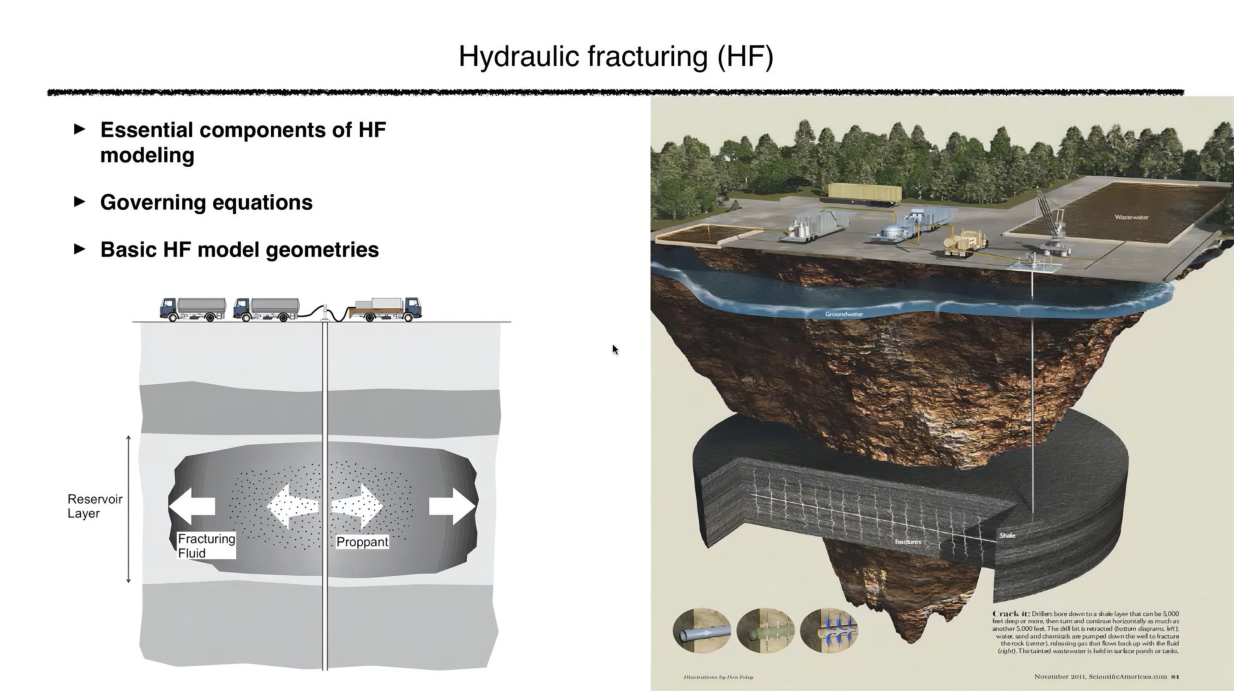
\includegraphics[width=\textwidth, page=1]{HF_slides_2021.pdf}

В двух словах разница между conventional и unconventional:

1) conventional -- то, что было, грубо говоря, до 2000-х годов -- вертикальная скважина, пласт, рвём гидроразрывом пласта, обычно одна трещина;

2) unconventional -- когда сланцы, например, то бурится горизонтальная скважина, проводится многостадийный ГРП (за одну стадию можем сделать несколько трещин (несколько портов), затем поставить перегородку, сделать ещё несколько трещин (портов) и так далее); можем также сделать несколько скважин.

Концептуально с точки зрения математики разницы между conventional и unconventional практически нет.
У нас либо одна трещина (conventional) или множество трещин (unconventional), т.е. с точки зрения моделирования unconventional моделировать дольше, сложнее.
Но повторюсь, что концептуально основная физика везде одинакова.

\subsection{Из чего состоит любая модель ГРП? Основные компоненты}

\includegraphics[width=\textwidth, page=2]{HF_slides_2022.pdf}

Основные компоненты любой модели гидроразрыва пласта:

1) закон сохранения жидкости; в 99\% случаев предполагается, что жидкость несжимаема, тогда выполняется закон сохранения объёма; но бывают случаи сжимаемых жидкостей (например, когда ГРП делают газом или делают пенный ГРП), тогда выполняется закон сохранения массы, т.е. закачиваемый объём жидкости равен объёму жидкости в трещине плюс утечки (трещину ГРП делаем в пористом резервуаре, поэтому есть утечки из трещины в резервуар -- в зависимости от пористости и других параметров утечки могут либо доминировать, либо нет: например, 90\% закачиваемой жидкости может утекать в пласт или наоборот оставаться в трещине);

2) уравнение течения жидкости в трещине;
допустим мы уже создали трещину в резервуаре (обычно она очень узкая и длинная: например, 1 сантиметр в ширину и порядка сотни метров в длину) и закачиваем в неё жидкость (которая часто бывает довольно вязкой), тогда у нас может быть существенное падение давления от скважины до кончика трещины (так как грубо говоря, всю эту жидкость нужно пропихнуть по всей трещине);
необходимы уравнения течения жидкости в зависимости от реологии жидкости;

3) равновесие (упругость) горной породы;
когда мы открываем трещину в упругом материале, то мы предполагаем, что порода линейно упругая (по крайней мере в первом приближении);
чтобы открыть трещину (т.е. просто открыть (как надуть шарик), а не распространить), нам необходимо приложить какое-то давление на стенки трещины (это давление и есть давление жидкости внутри трещины);
у нас получается некое распределение давления внутри трещины, и оно как-то неравномерно открывает эту трещину; чем сильнее мы хотим открыть трещину, тем больше должно быть давление жидкости внутри;

концептуальное уравнение: Fluid Pressure = Stress + Stiffness * FracWidth -- давление жидкости должно превысить напряжение в породе + жёсткость трещины (которая напрямую зависит от модуля Юнга породы), умноженную на среднее открытие трещины;
но большую часть составляет именно напряжение в породе, а дополнительное слагаемое с жёсткостью обычно много меньше (но тем не менее очень важно для моделирования); 

4) условие распространения трещины; грубо говоря, продолжая аналогию с шариком -- это критерий, при котором шарик лопнет; при достижении критического значения некого параметра около кончика трещины начнётся распространение трещины;

5) транспорт проппанта; это тоже очень важный компонент физики модели ГРП; высокопроводимый проппант нужен для того, чтобы при смыкании трещины ГРП остались проводимые каналы;
с точки зрения моделирования внутри жидкости течёт суспензия; обычно частицы проппанта (часто используется песок или керамический проппант с примерной плотностью 2.65 г/см$^3$) тяжелее жидкости (у воды плотность приблизительно 1 г/см$^3$), поэтому интересно моделировать процесс оседания проппанта.

\subsubsection{Модель утечки по Картеру}

\includegraphics[width=\textwidth, page=3]{HF_slides_2022.pdf}

Давайте рассмотрим модель утечки по Картеру.
Эта модель является доисторической для рассматриваемой области (для моделирования ГРП), её развил Картер ещё в 1956-1957 годах (тогда ещё только зарождался ГРП).
Первый коммерческий ГРП был сделан примерно в 1950-х годах.
Но тем не менее модель Картера и сейчас очень часто (почти повсеместно) используется при моделировании ГРП, потому что она очень простая и очень много физики в себе несёт.

В левом верхнем углу на слайде изображен рисунок (из PhD диссертации J. Adachi), на котором изображена область вблизи трещины.
Обычно жидкость ГРП состоит из основной жидкости (base fluid) и полимеров (их добавляют, чтобы химия или реология совпадала с той, которая нужна для дизайна ГРП, например, для нужной длины трещины или нужного транспорта проппанта и так далее).
Идея в том, что есть жидкость с полимерами.
Когда эта жидкость начинает фильтроваться в породу, то происходит следующее: в классической модели считаем, что полимеры большие, длинные и с трудом залезают в поровое пространство, т.е. полимеры в основном осаждаются на стенке трещины.
В итоге, образуется Filter Cake, который состоит из полимеров, добавляемых в жидкость ГРП.

Далее идёт Invaded Zone, в которой жидкость ГРП без полимеров затекает в породу и вымещает жидкость резервуара.

Далее идёт сам резервуар, в котором давление поднялось (так как мы вытеснили часть жидкости из Invaded Zone в резервуар).

Таким образом, концептуально график зависимости давления от вертикальной координаты $y$ выглядит следующим образом: на стенке трещины давление равно давлению жидкости, на бесконечности -- давление резервуара; 
давление жидкости больше, чем давление резервуара (иначе не смогли бы сгенерировать трещину ГРП);
есть падение давления на корке Filter Cake (предполагается, что оно линейное);
есть падение давления в Invaded Zone (тоже предполагается, что оно линейное);
и дальше есть падение давления в резервуаре.

Итак, есть три характерных падения давления.
Может быть так, что какое-то из них много меньше, чем другое; какое-то давление доминирует; может быть отсутствие Filter Cake (если в жидкости ГРП нет полимеров).
Но мы рассмотрим более общий случай и пройдёмся по уравнениям.

На слайде в левом нижнем углу представлена картина пористости сланца, полученная с помощью электронного микроскопа (маленькие поры, различные минералы и видно, что через эти поры жидкость утекает).
\\

Первым делом рассмотрим течение через корку Filter Cake.

Первое уравнение
\beq\label{FilterCake1}
g_c=\alpha\frac{dh_c}{dt}
\eeq
говорит нам о том, что скорость роста корки Filter Cake линейно пропорциональна количеству жидкости, утекаемому из трещины за единицу времени (или другими словами, линейно пропорциональна скорости утечки), а константа пропорциональности определяется экспериментально.
По сути $\alpha$ связана с концентрацией полимеров.

Второе уравнение 
\beq\label{FilterCake2}
g_c=\frac{\kappa_c}{\mu}\frac{\Delta p_{ci}}{h_c}
\eeq
это закон Дарси для течения жидкости через корку Filter Cake (полагаем, что падение давления на корке связано со скоростью утечек по линейному закону Дарси).

Приравнивая уравнения \eqref{FilterCake1} и \eqref{FilterCake2} и решая полученное обыкновенное дифференциальное уравнение, получаем
\beq
g_c=\frac{C_c}{\sqrt{t}}\,\,\,\,\,\,\,\,\,\,C_c=\sqrt{\frac{\alpha\kappa_c\Delta p_{ci}}{2\mu}}
\eeq
т.е. скорость утечек обратно пропорциональна $\sqrt{t}$.
\\

Далее рассмотрим следующую зону Invaded Zone.

Опять же предполагаем, что распределение давления линейное (довольно тонкая зона Invaded Zone) и выполняется линейный закон Дарси
\beq\label{InvadedZone1}
g_i=\frac{\kappa_r}{\mu}\frac{\Delta p_{ir}}{h_i}
\eeq

В качестве второго уравнения возьмём закон сохранения объёма
\beq\label{InvadedZone2}
g_i=\varphi\frac{dh_i}{dt}
\eeq
(т.е. объём жидкости, утекаемой из корки Filter Cake, определяет размер зоны Invaded Zone)

Приравнивая уравнения \eqref{InvadedZone1} и \eqref{InvadedZone2} и решая полученное обыкновенное дифференциальное уравнение, получаем
\beq
g_i=\frac{C_i}{\sqrt{t}}\,\,\,\,\,\,\,\,\,\,C_i=\sqrt{\frac{\varphi\kappa_r\Delta p_{ir}}{2\mu}}
\eeq
(подобно корке Filter Cake в Invaded Zone скорость утечек обратно пропорциональна $\sqrt{t}$).

\includegraphics[width=\textwidth, page=4]{HF_slides_2022.pdf}

Последний аспект физики здесь -- это поведение жидкости в резервуаре.
Одно из главных предположений модели Картера: предполагаем, что диффузия одномерная и перпендикулярная стенке трещины (т.е. рассматриваем изменение давления только по оси $y$).
Но на самом деле это не совсем так: если вы представите себе кончик трещины, то у него будет некая двумерная диффузия (или даже трёхмерная диффузия) вокруг кончика.

При каких условиях мы можем использовать предположение одномерности модели Картера?
Тогда, когда характерное расстояние, на котором осуществляется падение давления много меньше, чем длина трещины.
Вблизи кончика модель может не выполняться, но в где-то в середине трещины модель вполне себе применима.

Итак, рассматриваем одномерную модель, т.е. решаем уравнение одномерной диффузии, перпендикулярной стенке трещины.
Уравнение диффузии (диффузия в пороупругом материале) -- это опять таки закон Дарси плюс закон сохранения объёма.


\includegraphics[width=\textwidth, page=5]{HF_slides_2022.pdf}

\subsubsection{Течение жидкости в трещине ГРП}

\includegraphics[width=\textwidth, page=6]{HF_slides_2022.pdf}

Каждая модель ГРП должна включать в себя течение жидкости.
Обычно рассматривается следующая проблема.
Допустим мы открыли трещину, есть некое открытие трещины $w$ и течение вдоль оси $x$ (допустим, что она одномерное).
Открытие трещины обычно измеряется в миллиметрах, а длина трещины обычно составляет десятки или сотни метров. Т.е. получается очень узкая трещина и именно поэтому мы предполагаем, что в каждой точке трещины течение стационарно.
Т.е. необходимо решить стационарное уравнение Навье-Стокса.

\subsubsection{Равновесие (упругость) горной породы. Уравнение упругости}

\includegraphics[width=\textwidth, page=7]{HF_slides_2022.pdf}

Уравнение упругости.
Почему это сложно?
Потому что мы решаем уравнение упругости вокруг всей трещины.
Т.е. мы решаем уравнение упругости в 3D (или как минимум в 2D) вокруг трещины.
До этого у нас всё было одномерное: одномерные утечки Картера, одномерное течение жидкости в трещине.
А всё что одномерное, то просто.
Здесь же упругость как минимум двухмерная (а в большинстве случаев трёхмерная).
А в большинстве случаев решать трёхмерные задачи (особенно аналитически) не сильно весело, но можно.

В двух словах: пусть у нас есть несколько трещин (может быть одна трещина) и есть некоторое количество численных элементов, в которых трещина открыта.
Если приоткроем один из элементов ещё больше, то изменим поле напряжений везде в материале.
Т.е. у нас есть коэффициенты взаимодействия: как открытие любого из рассматриваемых элементов влияет на сжимающие напряжения в каждом другом элементе.

Аналогия с шариками: есть несколько тесно соединённых друг с другом шариков; мы надуваем один из шариков и в это же время все остальные сжимаются.

Т.е. суть уравнения упругости -- это посчитать коэффициенты взаимодействия (коэффициенты влияния) между элементами.
Ясно, что эти взаимодействия угасают с расстоянием, но тем не менее формально каждый элемент меняет поле напряжений во всём трёхмерном пространстве.

Обычно уравнение упругости относительно сложное (нелокальное) и оно обычно относительно медленно считается (в некоторых случаях по крайней мере).

Но я покажу вывод для плоской трещины (plain strain) -- предполагаем, что у нас двухмерная модель с некоторым открытием трещины.
Есть некое давление распределённое по оси $x$.
Есть сжимающие напряжения.
Мы выведем связь между распределением давления вдоль оси $x$, сжимающими напряжениями снаружи $\sigma_0$ и формой открытия трещины $w(x)$.
Нелокальная связь в том, что давление в точке зависит от интеграла открытия по всей трещине.
Т.е. изменение давления в произвольной ячейке приведёт к изменению давления по всей трещине.
Важная особенность в том, что интеграл в формуле гиперсингулярный и его нужно понимать в смысле главного значения.

Для планарной трещины аналогично.





\end{document}